%%%%%%%%%%%%%%%%%%%%%%%%%%%%%%%%%%%%%%%%%%%%%%%%%%%%%%%%%%%%%%%%%%%
%                                                                 %
%  GEANT manual in LaTeX form                                     %
%                                                                 %
%  Version 1.00                                                   %
%                                                                 %
%  Last Mod. 12 June 1993 1800   MG                               %
%                                                                 %
%%%%%%%%%%%%%%%%%%%%%%%%%%%%%%%%%%%%%%%%%%%%%%%%%%%%%%%%%%%%%%%%%%%
\Origin{L.Urb\'{a}n}
\Revision{G.Azuelos}
\Version{Geant 3.16}\Routid{PHYS351}
\Submitted{26.10.84}    \Revised{16.12.93}
\Makehead{Simulation of e+e- annihilation}
\section{Subroutines}
\Shubr{GANNI}{}
 
\Rind{GANNI} generates the annihilation of a positron into either one
or two photons. It uses the following input and output:
\begin{DLtt}{MMMMMMM}
\item[input:]  via common \FCind{/GCTRAK/}
\item[output:] via common \FCind{/GCKING/}
\end{DLtt}
The routine is called automatically from the tracking routine
\Rind{GTELEC}, when the positron reaches its interaction
point during the tracking.
\Shubr{GANNIR}{}
\Rind{GANNIR} generates the positron annihilation at rest. It is
called from the tracking routine \Rind{GTELEC}, if the positron
energy is below the cut-off energy {\tt CUTELE} in common block \FCind{/GCCUTS/}.
\section{Method }
The type of annihilation is sampled from the total cross-sections
for the annihilation into two photons and into one photon (see
section {\tt [PHYS350]}).
\subsubsection{Annihilation into two photons}
The differential cross-section of the two-photon
positron-electron annihilation can be written as 
\cite{bib-HEIT,bib-EGS3}:
\begin{equation}
\label{eq:phys351-1}
    \frac{d \sigma (Z, \epsilon)} {d \epsilon}=
       m \: a [S(a \epsilon) + S (a(1- \epsilon))]
\end{equation}
where $m$ is the  electron mass
$Z$ is the atomic number of the material. If we indicate with $E$ the
initial energy of the positron, with $r_{0}$ the classical electron
radius and with $k$ the energy of the less
energetic photon generated, we have:
\[
\begin{array}{LCL@{\hspace{4cm}}LCL}
\gamma   & = & \frac{E}{m} & a    & = & \gamma+1             \\
\epsilon & = & \frac{k}{E+m} & 
S(x)     & = & C_1 \left[ -1 + \frac{C_2}{x} -\frac{1} {x^2}\right]        \\
C_1 & = &  \frac{Z \pi r^2_0}{a(E-m)} & 
               C_2 & = & a + \frac{e \gamma}{a}
\end{array}
\]
The kinematical limits for the variable $\epsilon$ are:
\[
\epsilon_0 = \frac{1} {a+ \sqrt{\gamma^2 -1}}\leq \epsilon  \leq \frac{1} {2}
\]
Due to the symmetry of the formula (\ref{eq:phys351-1}) 
in $\epsilon$, the range of
$\epsilon$ can be expanded from ($\epsilon_0,1/2$) to
($\epsilon_0,1-\epsilon_0$)
and the second function $S$ can be eliminated from the formula.
Having done this, the differential
cross-section can be decomposed (apart from the normalisation) as:
\begin{equation}
\label{eq:phys351-2}
\frac{d \sigma} {d \epsilon}=\underbrace{\frac{1}{\ln
            \frac{1 - \epsilon_0}
            {\epsilon_0}}\frac{1}{\epsilon}}_{f(\epsilon)} 
\underbrace{\frac{(a^2 +2a-2)-a^2 \epsilon -\frac{1}{\epsilon }}
                  {a^2 -2\vphantom{{\ln \frac{1 - \epsilon_0}
                          {\epsilon_0}}}}}_{g(\epsilon)}
\end{equation}

\begin{figure}[hbt]
   \centering
   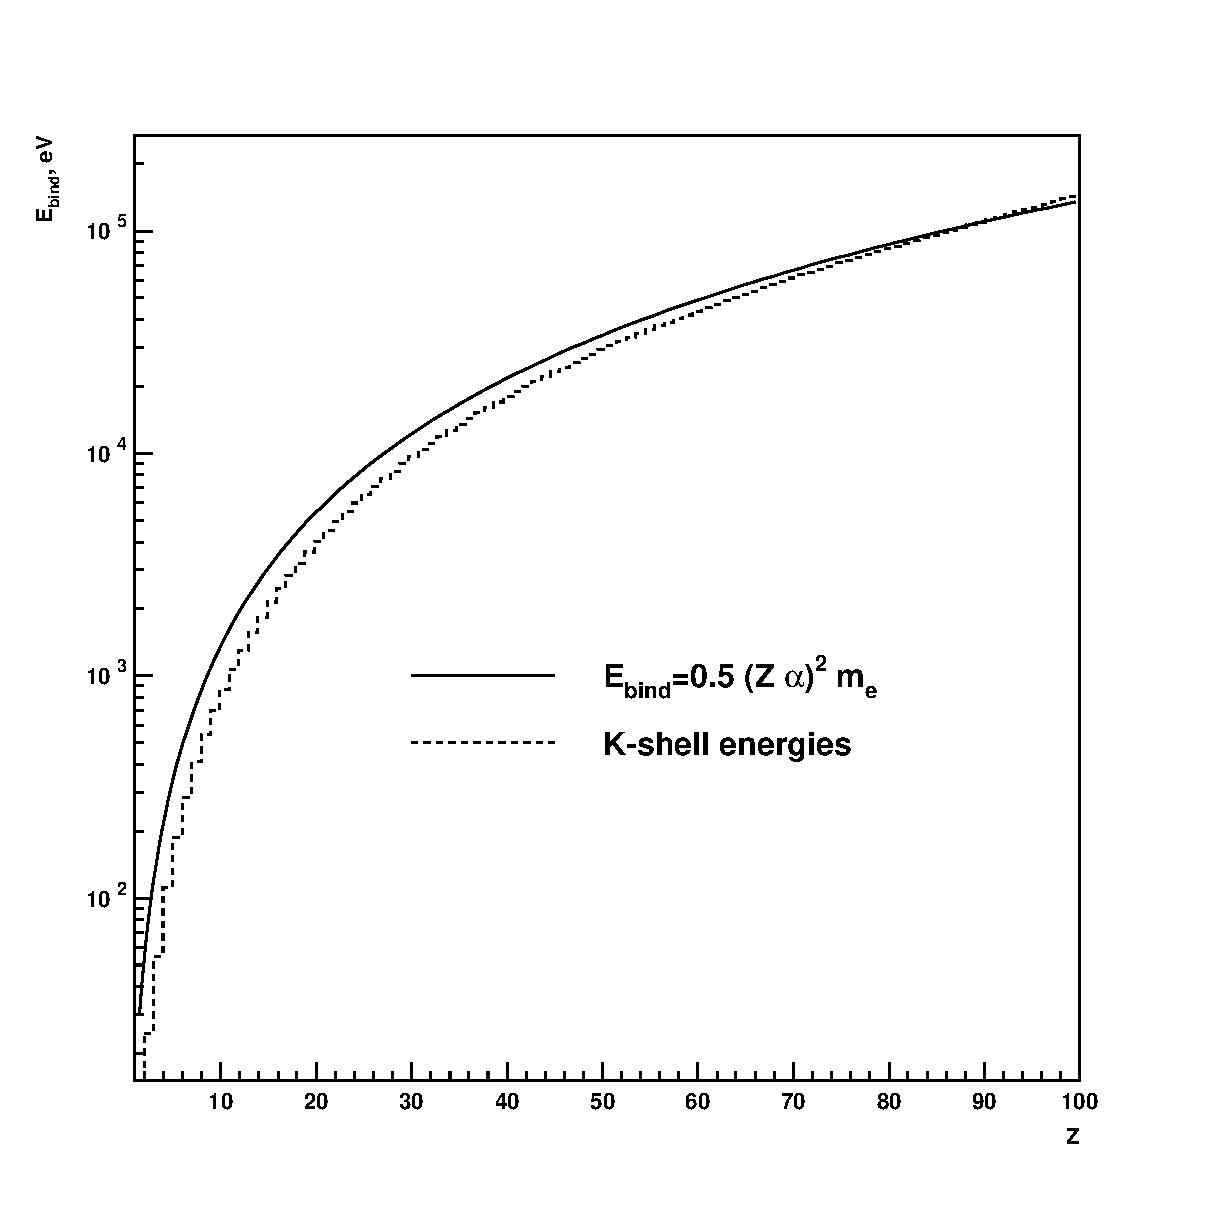
\epsfig{file=eps/phys351-1.eps,width=14cm}
   \caption{Comparison between the K-shell binding energies
            given by the expression in the text
            and the tabulated values. }
   \label{fg:phys351-1}
\end{figure}

Using the expression (\ref{eq:phys351-2}) with random numbers
$r_i \in ]0,1[, i=1,2$, the secondary photon energy is sampled by
the following steps:
\begin{enumerate}
\item sample $\epsilon$ from $f(\epsilon)$:
\begin{equation}
\epsilon =\epsilon_0 \exp  \left[ \ln \left(\frac{1- \epsilon_0}
{\epsilon_0}
          \right)  r_1  \right]
\end{equation}
\item
compute the rejection function $g(\epsilon)$ and
\begin{enumerate}
\item if $r_2 \leq g(\epsilon)$   accept $\epsilon$
\item if $r_1 > g(\epsilon)$  go back to 1.
\end{enumerate}
\end{enumerate}
After the successful sampling of $\epsilon$, the photon energy is computed as
 \begin{equation}
k = (E+m)\epsilon
\end{equation}
and then \Rind{GANNI} generates the polar angles of the photon with respect
to an axis defined by the momentum of the positron. The azimuthal angle
$\Phi$ is generated isotropically and $\Theta$ is computed from the
energy-momentum conservation. With this information, the momentum
vector of both photons can be calculated and transformed into the {\tt GEANT}
coordinate system.
 
The routine \Rind{GANNIR} treates the special case when a positron falls
below the cut-off energy ({\tt CUTELE} in 
common block \FCind{/GCCUTS/}) before annihilating.
In this case, it is assumed that the positron comes to rest before annihilating.
\Rind{GANNIR} generates two photons with energy $k=m$. The
angular distribution is isotropic.
\subsubsection{Annihilation into one photon}
The generated photon is assumed to be collinear with the positron.
Its energy will be
\begin{equation}
k = E + m_e - E_{bind}
\end{equation}
where $E_{bind}$ is the binding energy of the K-shell electron.
It can be estimated as follows
\begin{equation}
\label{eq:phys315-1}
E_{bind} = 0.5 (Z \, \alpha )^2  \, m_e
\end{equation}
where $\alpha$ is the fine stucture constant. The comparison
of this expression with the experimental data from
\cite{bib-XRAY} is shown in figure \ref{fg:phys351-1}.

\section{Restrictions}
\begin{enumerate}
\item
The annihilation processes producing three or more photons are
ignored, because these processes are negligible compared to the 
annihilation into two photons~\cite{bib-EGS3,bib-MES1};
\item
In calculating the process it is assumed that the atomic electron initially
is free and at rest. This is the usual assumption used in shower programs
\cite{bib-EGS3};
\end {enumerate}
